\documentclass{report}
\usepackage{blindtext}
\usepackage{geometry}
\usepackage{circuitikz}

%python code
\usepackage{listings}
\usepackage{xcolor}
\definecolor{codegreen}{rgb}{0,0.6,0}
\definecolor{codegray}{rgb}{0.5,0.5,0.5}
\definecolor{codepurple}{rgb}{0.58,0,0.82}
\definecolor{backcolour}{rgb}{0.95,0.95,0.92}
\lstdefinestyle{mystyle}{
    backgroundcolor=\color{backcolour},   
    commentstyle=\color{codegreen},
    keywordstyle=\color{magenta},
    numberstyle=\tiny\color{codegray},
    stringstyle=\color{codepurple},
    basicstyle=\ttfamily\footnotesize,
    breakatwhitespace=false,         
    breaklines=true,                 
    captionpos=b,                    
    keepspaces=true,                 
    numbers=left,                    
    numbersep=5pt,                  
    showspaces=false,                
    showstringspaces=false,
    showtabs=false,                  
    tabsize=2
}
\lstset{style=mystyle}

\geometry{
 a4paper
}
%---------------------------------------------
\usepackage{xcolor}
\usepackage{tcolorbox}
%\usepackage[resetlabels,labeled]{multibib}
%\newcites{CitedFigure}{Cited Figures}
%---------------------------------------------

%------
% Font
%------
\pagenumbering{Roman}
\usepackage[utf8]{inputenc} % allows non-ascii input characters
\usepackage{lettrine}

\usepackage{slashed}
\usepackage{braket}

%-----------------------
% Proper word splitting
%-----------------------
\usepackage[english]{babel} 
\usepackage[parfill]{parskip} 

% Mathematics
%-------------
\usepackage{amsmath}
\usepackage{slashed}
\usepackage{amsfonts}
\usepackage{stackengine}
\def\delequal{\mathrel{\ensurestackMath{\stackon[1pt]{=}{\scriptscriptstyle\Delta}}}}
\usepackage{mathrsfs}

%---------
% Figures
%---------
\graphicspath{{./figures/}}

%-----------------------
% Bibliography settings
%-----------------------
\usepackage{cite}

% Hyperreferences
%-----------------
\usepackage{hyperref}

%--------------------------------------------------
% Quotes
%--------------------------------------------------
\makeatletter
\renewcommand{\@chapapp}{}
\newenvironment{chapquote}[2][2em]
  {\setlength{\@tempdima}{#1}%
   \def\chapquote@author{#2}%
   \parshape 1 \@tempdima \dimexpr\textwidth-2\@tempdima\relax%
   \itshape}
  {\par\normalfont\hfill--\ \chapquote@author\hspace*{\@tempdima}\par\bigskip}
\makeatother
%----------------------
% Input for title page
%----------------------

\begin{document}

% =====================================================================
% Cover
% =====================================================================

%  Titelblad

% Opmerking: gaat uit van een \baselinestretch waarde van 1.5 (die moet
% ingesteld worden voor het begin van de document environment)

\begin{titlepage}

% \textwidth en \textheight hier aanpassen blijkt niet te werken

\fontsize{12pt}{14pt}
\selectfont

\begin{center}


\includegraphics[height=4cm]{figures/ruglogo.pdf}

\vspace{0.5cm}

Royal Military Academy\\
Research Group Plasma Physics

\vspace{3.5cm}

\fontseries{bx}
\fontsize{17.28pt}{21pt}
\selectfont
Internal report:\\
ICRH automatic matching system on TOMAS

\fontseries{m}
\fontsize{12pt}{14pt}
\selectfont

\vspace{.6cm}


\vspace{.4cm}

Arthur Adriaens

\vspace{3.5cm}

\end{center}
\end{titlepage}


% =====================================================================
% Front matter
% =====================================================================

\shipout\null
\newpage

% ------------ TABLE OF CONTENTS ---------
{\hypersetup{hidelinks}\tableofcontents} % hide link color in toc
\newpage

% =====================================================================
% Main matter
% =====================================================================

\pagenumbering{arabic}
\chapter{Overview}
\section{Introduction}
This work aims to be a succesful implementation of an automatic matching
algorithm for the Ion Cyclotron Resonance Heating (ICRH) antennna, a circuit
drawing of this matching system is shown in figure \ref{fig:Circuit}.  The antennae are
facing a plasma with ever changing conditions: the density, temperature and
even species (He/H/Ar) may vary; As such the capacitance of the various capacitors
have to be varied every time the conditions change as to maximize power transfer.\\

At the time of writing this is carried out manually by first lowering the
current going to the antenna by adjusting $C_a$, then varying capacitances of $C_p$ and
$C_s$, doing a frequency sweep and looking where the power transferred is
maximal (i.e the measured reflected power is minimal), if the frequency at
which this happens coincides with the required frequency then we stop
adjusting $C_s$ and $C_p$ and heighten the current flowing to the antenna using $C_a$.
\begin{figure}[h]
\centering
\begin{circuitikz}[european] \draw
  (0,0) to [short, *-] (4,0)
  (4,0) to [vC, l=$C_p$] (4,4)
  (4,0)  to [short, *-] (6,0)
  node[ground] (6,0)
  to [short, *-] (8,0)
  to [short, *-] (12,0)
  (0,0) node[below]{$B$} to [open, v^>=$P_s$]  (0,4) 
  (0,4) node[above]{$A$} to [short, *- ,i=$i_{in}$] (1,4) 
  (4,4) to [short, *-] (0,4)
  (4,4) node[above]{$C$} to [vC, l=$C_{s}$] (8,4) 
  (12,0) to [vC, l=$C_{a}$] (12,4) 
  (8,4) node[above]{$E$} to [R, l=$Z_{Ant,s}$]  (12,4)
  (12,4) node[above]{$G$}
  (4,0) node[below]{$D$}
  (8,0) node[below]{$F$}
  (12,0) node[below]{$H$}
  (8,0) to [R, l=$Z_{Ant,p}$]  (8,4);
  %\node at (1.5,2) (loop1) {$\ \ \qquad1$}
  %\draw [->] (loop1.south)arc(-160:160:0.5);
  %\node at (5.5,2) (loop2) {$\ \ \qquad2$}
  %\draw [->] (loop2.south)arc(-160:160:0.5);
  %\node at (9.5,2) (loop3) {$\ \ \qquad3$}
  %\draw [->] (loop3.south)arc(-160:160:0.5);
\end{circuitikz}
\caption{
The Power input is marked $P_s$, the antenna can be described as having a
parallel impedence $Z_{Ant,p}$ and a series impedence $Z_{Ant,s}$. The power
input is assumed to have an entry impedence of $Z_0=50\Omega$ and to match the
circuit we can play around with the variable parallel matching $C_p$, the
series matching $C_s$ and the pre-matching $C_a$ capacitors}
\label{fig:Circuit}
\end{figure}

\section{Previous work}
Work has been done on this previously by F. Fasseur\cite{Saussez}, which lays
out a good exposition on the system, how changing the various capacitors affects the system 
and which capacitance values of $C_a$ result in a matchable system.\\

K. Elinck continued on this work by implementing a neural network and training it on simulated data\cite{Gen2019},
we question wether the simulated training corresponds well with the experiment and if it's even needed to make the algorithm
so complex (as e.g TEXTOR's circuit worked fine\cite{DURODIE1993477} which was just a simple linear algorithm) and as such 
we won't go into detail on his work.
\section{system}
To understand how to, in practice, implement an algorithm, the interconnectedness of the ICRH system needs to be discussed:
A computer which we'll henceforth call pc1 is connected to an Arduino which can modify the capacitance of the capacitors
with steppermotors. pc1 is also connected to the ICRH amplifier
making it possible to select the power.

The DAQ, however, is a second computer: pc2. We can thus set the various
parameters on pc1 but only see what they imply on pc2, making it necessary to
transfer data between the two, which makes the automatic matching a little more
complex.

%\chapter{AC relations}
As we're dealing with an AC circuit we'll of course use phasors as to make Kirchoffs
laws hold, phasors will be indicated with a hat.
This is going to be quite a long derivation, so buckle up!\\
\section{Derivation of phasor relations}
loop 1 implies
\begin{eqnarray}
	\hat{V}_{AB} - \hat{V}_{CD} &= 0\\
	\hat{V}_{AB} + \frac{i}{\omega C_p} \hat{I}_{CD} &= 0\\
	i \omega C_p\hat{V}_{AB} &= \hat{I}_{CD}
\end{eqnarray}
Loop 2 implies
\begin{eqnarray}
	-\hat{V}_{CD} - 	\frac{i}{\omega C_s} \hat{I}_{CE} + \hat{V}_{AP} &= 0\\
	-\hat{V}_{AB} - 	\frac{i}{\omega C_s}(\hat{I}_{in} - \hat{I}_{CD}) + \hat{V}_{AP}&= 0\\
	-\hat{V}_{AB} - 	\frac{i}{\omega C_s}\left(\frac{\hat{V}_{AB}}{Z_0} - i\omega C_p\hat{V}_{AB}\right) + \hat{V}_{AP}&= 0\\
-\hat{V}_{AB}\left(1 + 	\frac{i}{\omega C_s Z_0} + \frac{C_p}{C_s}\right) + \hat{V}_{AP}&= 0\\
	\hat{V}_{AB}\left(\frac{i}{\omega C_s Z_0} + \frac{C_s + C_p}{C_s}\right) &= \hat{V}_{AP}\\
\end{eqnarray}
So we now have a relation between the phasor of the input power and the one on the parallel part of the antenna:
\begin{equation}
	\boxed{\hat{V}_{AP}=\hat{V}_{AB}\left(\frac{i}{\omega C_s Z_0} + \frac{C_s + C_p}{C_s}\right)} \label{eqn:APphasor}
\end{equation}
Loop 3 implies
\begin{eqnarray}
	\hat{V}_{AS} - \frac{i}{\omega C_a} \hat{I}_{EG} - \hat{V}_{AP} &= 0\\
	\hat{V}_{AS}  - \hat{V}_{AP} &= \frac{i}{\omega C_a} \hat{I}_{EG}\\
	-i\omega C_a\left( \hat{V}_{AS}  - \hat{V}_{AP}\right) &= \hat{I}_{EG}
	\label{eqn:loop3}
\end{eqnarray}
Now if we take a zoomed out look at the circuit we can see another loop: loop 4, the outer part of the circuit.
Note that this carries no additional information as loops 1 + 2 + 3 equal this loop but we'll go through it anyways
as a consistency check:\\
Loop 4 implies:
\begin{eqnarray}
	&\hat{V}_a + \hat{V}_{AS} + \hat{V}_s - \hat{V}_{AB} = 0\\
	&-\frac{i}{\omega C_a}\hat{I}_{GH} + \hat{V}_{AS} - \frac{i}{\omega C_s} \hat{I}_{CE} - \hat{V}_{AB} = 0\\
	&-\frac{i}{\omega C_a}\hat{I}_{EG} + \hat{V}_{AS} - \frac{i}{\omega C_s} \hat{I}_{CE} - \hat{V}_{AB} = 0\\
	&-\left( \hat{V}_{AS}  - \hat{V}_{AP}\right) + \hat{V}_{AS} - \frac{i}{\omega C_s}\left(\frac{\hat{V}_{AB}}{Z_0} + i\omega C_p\hat{V}_{AB}\right) - \hat{V}_{AB} = 0\\
	&\hat{V}_{AP} - \frac{i}{\omega C_s}\left(\frac{\hat{V}_{AB}}{Z_0} + i\omega C_p\hat{V}_{AB}\right) - \hat{V}_{AB} = 0
\end{eqnarray}
Which we have previously encountered, proving that we're consistent.\\
Let's continue on equation \ref{eqn:loop3};
We have that (I couldn't find any relation $f(\hat{V}_{AB}) = \hat{I}_{EG}$):
\begin{equation}
	\hat{I}_{EG} = \frac{\hat{V}_{AS}}{Z_{AS}}
\end{equation}
So
\begin{eqnarray}
	\hat{V}_{AS}\left(1  - \frac{i}{\omega C_a Z_{AS}}\right) &= \hat{V}_{AP}\\
\end{eqnarray}
And using equation \ref{eqn:APphasor} we thus get:
\begin{eqnarray}
	\hat{V}_{AS}\left(1  - \frac{i}{\omega C_a Z_{AS}}\right) &= \hat{V}_{AB}\left(\frac{i}{\omega C_s Z_0} + \frac{C_s + C_p}{C_s}\right)\\
	\hat{V}_{AS} &= \hat{V}_{AB}\frac{\frac{i}{\omega C_s Z_0} + \frac{C_s + C_p}{C_s}}{1  - \frac{i}{\omega C_a Z_{AS}}}\\
\end{eqnarray}
I.e
\begin{equation}
	\hat{V}_{AS} = \hat{V}_{AB}\frac{i C_a Z_{AS} + \omega C_a Z_{AS} Z_0(C_s + C_p)}{\omega C_a C_s Z_{AS} Z_0 - iC_s Z_0}
\end{equation}
Let's split this up into an imaginary and real part:
\begin{eqnarray}
\hat{V}_{AS} &= \hat{V}_{AB}\frac{i C_a Z_{AS} + \omega C_a Z_{AS} Z_0(C_s + C_p)}{\omega C_a C_s Z_{AS} Z_0 - iC_s Z_0}\\
\hat{V}_{AS} &= \hat{V}_{AB}\frac{\left[i C_a Z_{AS} + \omega C_a Z_{AS} Z_0(C_s + C_p)\right](\omega C_a C_s Z_{AS} Z_0 + iC_s Z_0)}{(\omega C_a C_s Z_{AS} Z_0 - iC_s Z_0)(\omega C_a C_s Z_{AS} Z_0 + iC_s Z_0)}\\
\hat{V}_{AS} &= \hat{V}_{AB}\frac{\left[i C_a Z_{AS} + \omega C_a Z_{AS} Z_0(C_s + C_p)\right](\omega C_a C_s Z_{AS} Z_0 + iC_s Z_0)}{(\omega C_a C_s Z_{AS} Z_0)^2 + (C_s Z_0)^2}\\
\hat{V}_{AS} &= \hat{V}_{AB}(C_a C_s Z_{AS} Z_0)\frac{\omega^2 C_a Z_{AS} Z_0(C_s + C_p) - 1 + i\omega  \left[C_a Z_{AS} + Z_0(C_s + C_p)\right]}{(\omega C_a C_s Z_{AS} Z_0)^2 + (C_s Z_0)^2}\\
\hat{V}_{AS} &= \hat{V}_{AB}(C_a Z_{AS} )\frac{\omega^2 C_a Z_{AS} Z_0(C_s + C_p) - 1 + i\omega  \left[C_a Z_{AS} + Z_0(C_s + C_p)\right]}{(\omega C_a^2 C_s Z_{AS}^2 Z_0) + (C_s Z_0)}\\
\hat{V}_{AS} &= \hat{V}_{AB}(C_a Z_{AS})\left[\frac{\omega^2 C_a Z_{AS} Z_0(C_s + C_p)}{(\omega C_a^2 C_s Z_{AS}^2 Z_0) + (C_s Z_0)} + i\frac{\omega  \left[C_a Z_{AS} + Z_0(C_s + C_p)\right]}{(\omega C_a^2 C_s Z_{AS}^2 Z_0) + (C_s Z_0)}\right]\\
\hat{V}_{AS} &= \hat{V}_{AB}\left[\frac{\omega^2 C_a Z_{AS} Z_0(C_s + C_p)}{(\omega C_a C_s Z_{AS} Z_0) + (\frac{C_s Z_0}{C_a Z_{AS}})} + i\frac{\omega  \left[C_a Z_{AS} + Z_0(C_s + C_p)\right]}{(\omega C_a C_s Z_{AS} Z_0) + (\frac{C_s Z_0}{C_a Z_{AS}})}\right]
\end{eqnarray}\\
i.e
\begin{equation}
	\boxed{
	\hat{V}_{AS} = \hat{V}_{AB}\left[\frac{\omega^2 C_a Z_{AS} Z_0(C_s + C_p)}{(\omega C_a C_s Z_{AS} Z_0) + (\frac{C_s Z_0}{C_a Z_{AS}})} + i\frac{\omega  \left[C_a Z_{AS} + Z_0(C_s + C_p)\right]}{(\omega C_a C_s Z_{AS} Z_0) + (\frac{C_s Z_0}{C_a Z_{AS}})}\right]}
\end{equation}
Which is quite a long and difficult equation, we can however make a little approximation, as the capacitors are in the pF range and the frequency is in the MHz range
we have that
\begin{equation}
	\omega C_a C_s Z_{AS} Z_0 \ll \frac{C_s Z_0}{C_a Z_{AS}}
\end{equation}
so
\begin{eqnarray}
	\hat{V}_{AS} &\approx \hat{V}_{AB}\left[\frac{\omega^2 C_a Z_{AS} Z_0(C_s + C_p)}{(\frac{C_s Z_0}{C_a Z_{AS}})} + i\frac{\omega  \left[C_a Z_{AS} + Z_0(C_s + C_p)\right]}{(\frac{C_s Z_0}{C_a Z_{AS}})}\right]\\
	\hat{V}_{AS} &\approx \hat{V}_{AB}\left[\frac{\omega^2 C_a^2 Z_{AS}^2 Z_0(C_s + C_p)}{C_s Z_0} + i\frac{\omega C_a Z_{AS} \left[C_a Z_{AS} + Z_0(C_s + C_p)\right]}{C_s Z_0}\right]\\
	\hat{V}_{AS} &\approx \hat{V}_{AB}\frac{\omega C_a Z_{AS}}{C_s Z_0}\left[\omega C_a Z_{AS} Z_0(C_s + C_p) + i\left[C_a Z_{AS} + Z_0(C_s + C_p)\right]\right]\\
	\hat{V}_{AS} &\approx \hat{V}_{AB}\frac{\omega C_a Z_{AS}}{C_s}\left[\omega C_a Z_{AS} (C_s + C_p) + i\left[C_a \left(\frac{Z_{AS}}{Z_0}\right) + (C_s + C_p)\right]\right]
	\label{eqn:AS_phasor}
\end{eqnarray}
Note that this equation also depends on $Z_{AS}$ which we don't know.
We'll later on see wether we can do something about this.
\newpage
\section{Derivation of measurables}
We'll now convert the phasors to measurables, as
\begin{equation}
	\hat{V}_1 = (a + bi)\hat{V}_2 \implies V_1 = V_0 \sqrt{a^2 + b^2} \cos{(\omega t + \phi)}
\end{equation}
With
\begin{equation}
	\phi = \arctan{\left(\frac{b}{a}\right)}
\end{equation}
From equation \ref{eqn:APphasor}, we have:
\begin{equation}
	V_{AP} = V_0\sqrt{\left(\frac{C_s + C_p}{C_s}\right)^2 + \left(\frac{1}{\omega C_s Z_0}\right)^2}\cos{\left[\omega t + \arctan{\left(\frac{1}{\omega Z_0 (C_S + C_p)}\right)\right]}}
\end{equation}
So resonance over the parallel component of the antenna occurs when 
\begin{equation}
	1 + 2\frac{C_p}{C_s} + \left(\frac{C_p}{C_s}\right)^2 + \frac{1}{(\omega C_s Z_0)^2 }\label{eqn:ResonanceForPar}
\end{equation}
is maximal, in other words, given some angular frequency $\omega$, we may vary $C_p$ and $C_s$ to maximize the power transfer to the parallel component. How this varies
is shown below on a log scale, as can be seen, the ideal position is having $C_s$ as close to 0pF as possible and $C_p$ as close to 1000pF, as is expected when looking
at the circuit. The problem is of course that we don't just need to maximize the power in the parallel system but also in the serial system.
\begin{figure}[ht]
	\centering
	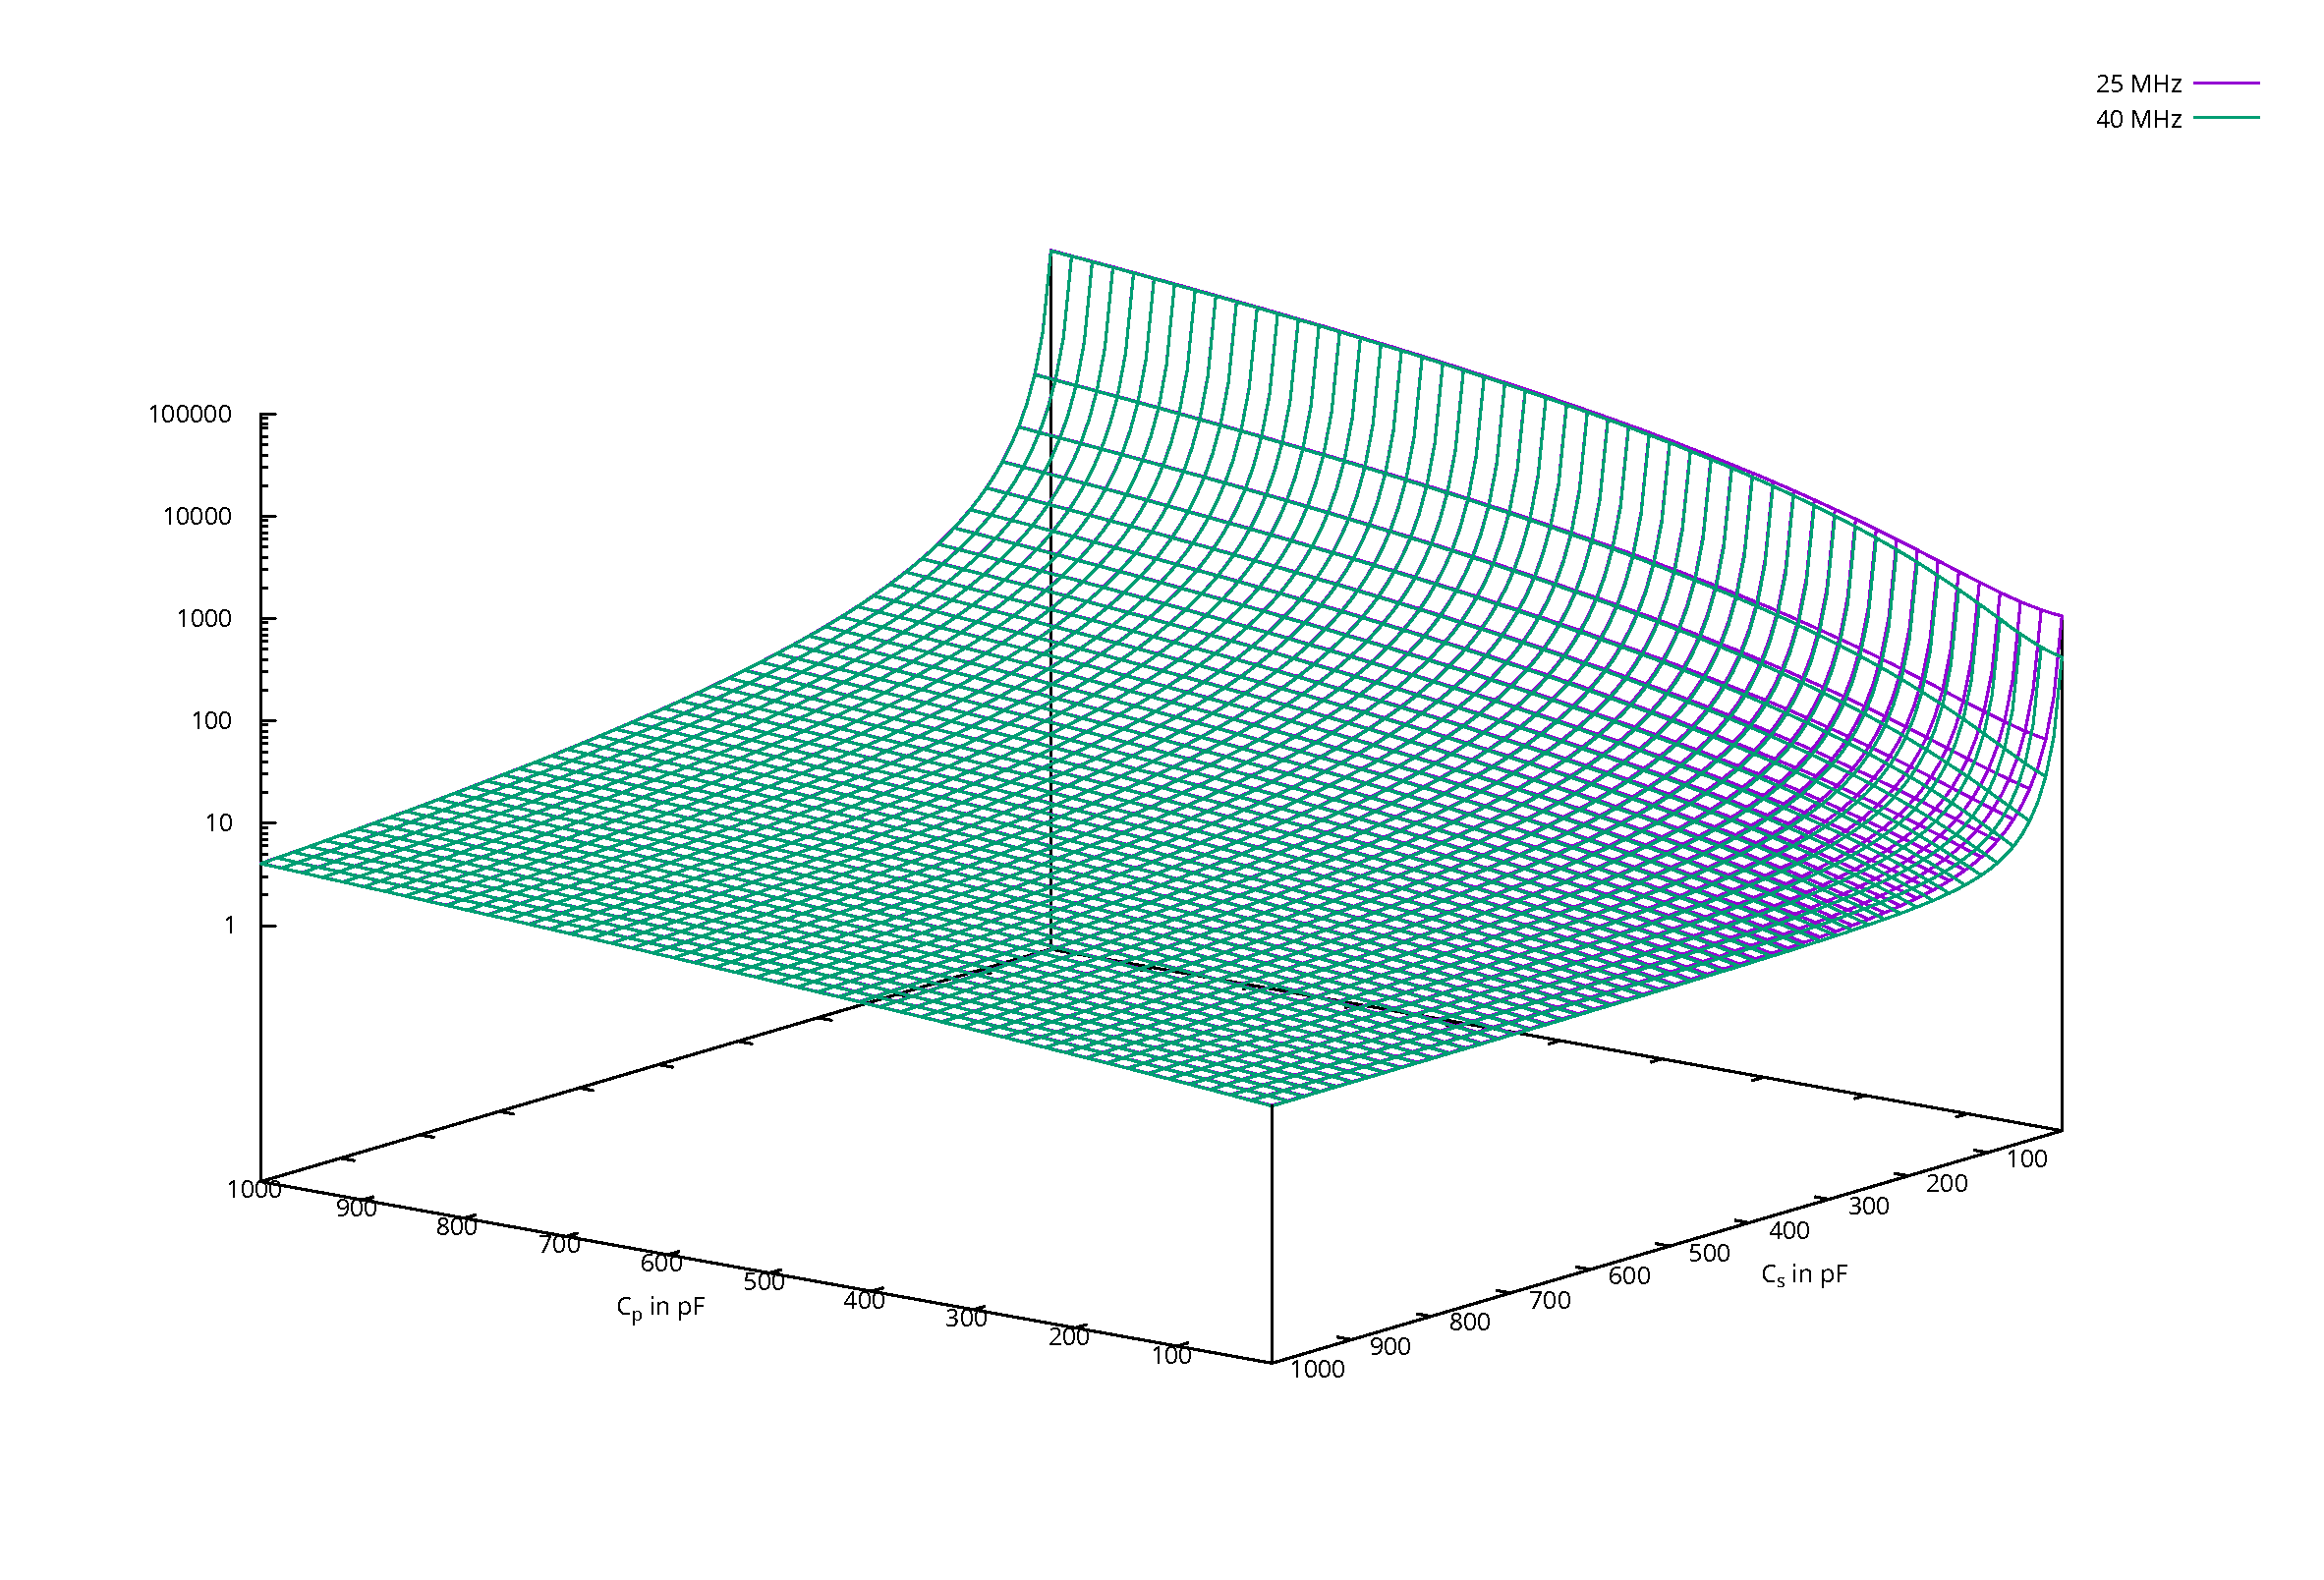
\includegraphics[width=0.9\textwidth]{ParallelMatching.pdf}
\end{figure}\\
From equation \ref{eqn:AS_phasor} we have a phase
\begin{equation}
	\phi = \arctan{\left(\frac{C_a \left(\frac{Z_{AS}}{Z_0}\right) + C_s + C_p}{\omega C_a Z_{AS} (C_s + C_p)}\right)}
\end{equation}
As we somewhat know $\omega$, $C_a$, $C_s$ and $C_p$, by measuring the phase we can thus infer $Z_{AS}$. Now resonance occurs when
\begin{equation}
	\left(\frac{\omega C_a Z_{AS}}{C_s}\right)^2\left[\left(\omega C_a Z_{AS} (C_s + C_p)\right)^2 + \left(C_a \left(\frac{Z_{AS}}{Z_0}\right) + (C_s + C_p)\right)^2\right]
\end{equation}
Is maximal, we'll thus need to maximize the following two equations:\\

\begin{equation}
	\boxed{1 + 2\frac{C_p}{C_s} + \left(\frac{C_p}{C_s}\right)^2 + \frac{1}{(\omega C_s Z_0)^2 }}
\end{equation}
and
\begin{equation}
	\boxed{\left(\frac{\omega C_a Z_{AS}}{C_s}\right)^2\left[\left(\omega C_a Z_{AS} (C_s + C_p)\right)^2 + \left(C_a \left(\frac{Z_{AS}}{Z_0}\right) + (C_s + C_p)\right)^2\right]}
\end{equation}

To obtain resonance over the antenna.

\include{MainMatter/Fred.tex}
%\chapter{Frequency sweep matching}
\section{Outline of the system}
Computer 1 will set the capacitors $C_p$,$C_s$ and $C_a$ on capacitances
\begin{eqnarray}
	a &\in (\text{35pF},\text{1000pF})\\
	s &\in (\text{25pF},\text{1000pF})\\
	p &\in (\text{7pF},\text{1000pF})
\end{eqnarray}
And start a \textit{Frequency sweep} i.e vary the frequency over some interval
(relevant to ICRH, e.g 10-55MHz), keeping the power constant.\\ The waveguide
is equipped with a differential coupler, making it possible to measure the
amplitude of the reflected signal. This way we can see it make a dip at the
"matched" frequency, let's for now quantify the discrepency between the
required/requested frequency $f_r$ and the matched frequency $f_m$ using
\begin{equation}
	\Delta f^2 = f_m^2 - f_r^2
\end{equation}
Our goal is thus to minimize $\Delta f$ (note that we throw some information
away by making it positive definite, this won't become a problem as will be shown),
making the matched frequency corresponding to the system as close as possible
to the frequency we want. To do this we'll send the frequency sweep data over
from computer 2 (DAQ) to computer 1 (GUI), find $f_m$ by seeking the minimum of
the reflected signal, compute $\Delta f$, feed this into a program which
manipulates the capacitors to try and bring this value to zero, and repeat.
This system is shown in figure 
\ref{fig:system}.
\begin{figure}[h]
	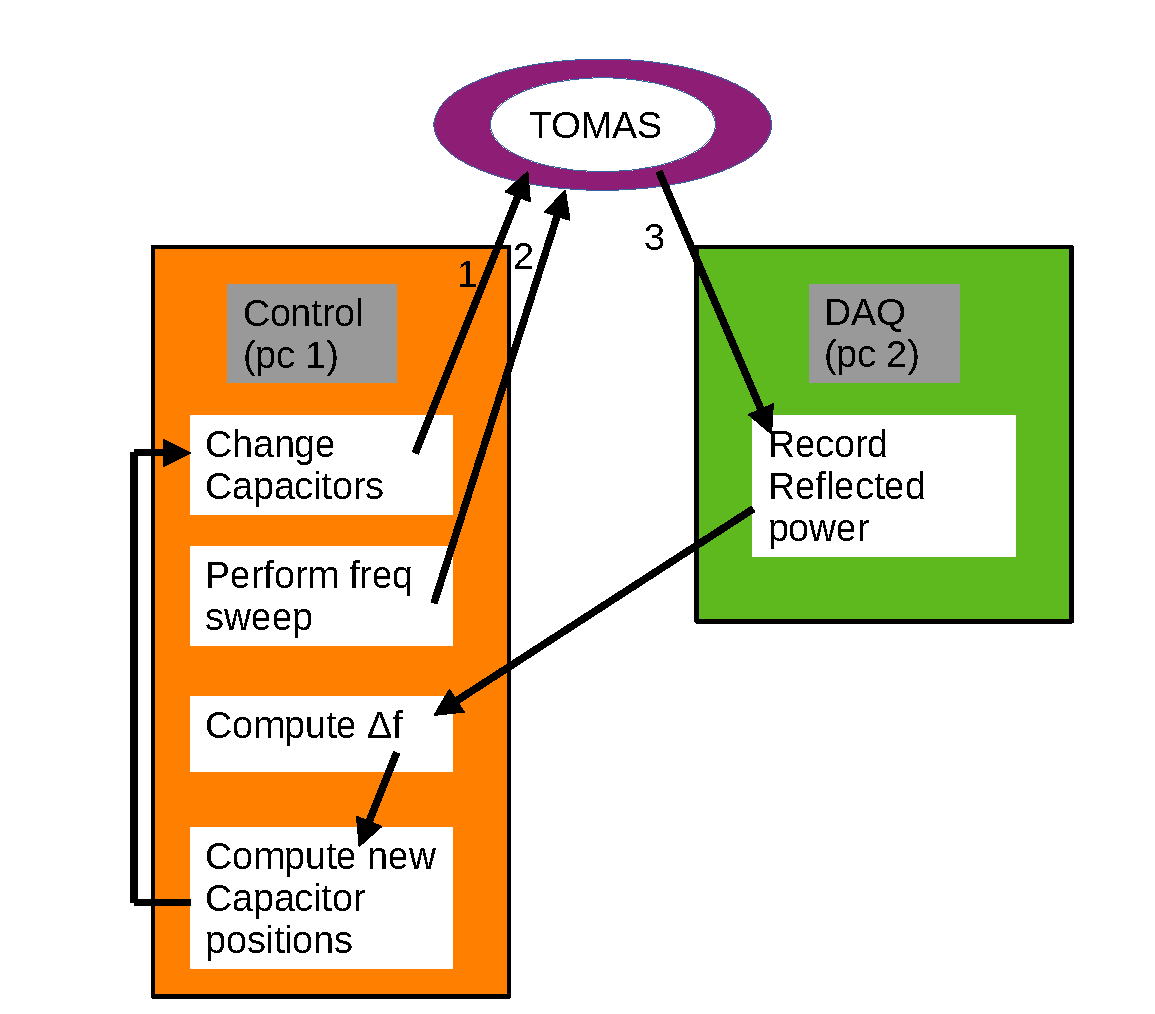
\includegraphics[width=\textwidth]{System.pdf}
	\caption{Overview of the system, pc2 will communicate with pc1 through TCP/IP}
	\label{fig:system}
\end{figure}
\section{Algorithm}
It's all well and good to think out a way to change everything in steps but the biggest problem
is still the same: how should the capacitances be chosen i.f.o $\Delta f$?
I.e what does the 3-dimensional function
\begin{equation}
	\vec{f}(\Delta f) = \vec{C} = \begin{bmatrix}
a\\
p\\
s\\
\end{bmatrix}
\end{equation}
look like? Well let's start by eliminating the variable a as we'll just lower
it initially and heighten it after the matching is complete (hoping this
doesn't change the matched frequency too much). This leaves us with one input
for 2 outputs, we can however, using a a new power meter, also record the phase
of the reflected power $\Gamma_\phi$.  We can thus change the function to:
\begin{equation}
	\vec{f}(\Delta f, \Gamma_\phi) = 
	\begin{bmatrix}
	p\\
	s\\
	\end{bmatrix}
\end{equation}
Let's start by trying out a simple 


% =====================================================================
% End matter
% =====================================================================

\bibliographystyle{IEEEtran}
\bibliography{IEEEabrv,Bibliography/sources}

\end{document}
